\documentclass{beamer}
\usepackage{amsmath}
\usepackage{enumitem}
\mode<presentation>{\usetheme{Malmoe}}

%%preamble
\newcommand{\ignore}[1]{}
\newcommand*{\diff}{\mathsf{d}}
\newcommand{\some}{{\color{red} something}}
\renewcommand{\vec}[1]{\mathbf{#1}}




\title{Free energy of a liquid}
\author{Brenden Vischer}



\begin{document}
\setbeamercolor{whitebox}{bg=gray!40}

%%main

\begin{frame}
	\titlepage
\end{frame}

%% Body
\AtBeginSection[]
{\begin{frame}{Table of Contents}
	\tableofcontents[currentsection]
\end{frame}}

\section*{Introduction}
\subsection*{Free energy}
\begin{frame}{What is free energy?}
		\begin{columns}
			\column{.5\textwidth}
				Legendre Transform: 
				\begin{align*}
				 	F &= U - T\,S\\
				 	\diff F &= - S\, \diff T + P\, \diff V
				\end{align*}
				Statistical Mechanics: 
				\begin{align*}
					F &= - k_B T \ln \mathcal Z
				\end{align*}

			\column{.5\textwidth}
			Why Helmholtz and not Gibbs?
			\begin{itemize}
				\item Temperature and volume natural to control (pressure less so)
				\item Entropy is derivative at constant volume rather than constant pressure
				\item Statistical mechanics definition of $F$ - microscopic systems  
			\end{itemize}
		\end{columns}
\end{frame}

\subsection*{Why separation?}
\begin{frame}{Why is separation important?}
		\begin{columns}[t, onlytextwidth]
			\column{.5\textwidth}
			\begin{itemize}[noitemsep]
				\item (something about systems being able to be separated - enumerating energies, then separating partition function, then stuff) 
			\end{itemize}
			\column{.5\textwidth}
			Statistical Associating Fluid Theory 
			\begin{align*}
				\frac{F}{N k_B T} &= ~\frac{F_{id}}{N k_B T} + \frac{F_{mono}}{N k_B T} \\
				&\quad +\frac{F_{assoc}}{N k_B T} + \frac{F_{chain}}{N k_B T}  
			\end{align*}
		\end{columns}
\end{frame}

\subsection*{Partition function}
\begin{frame}
	\begin{itemize}
		\item 
			\begin{align*} Z &= \sum_E^{\text{\tiny Energies}} D(E) 	
			\exp\left(-\frac{E}{k_b T}\right)
			\end{align*}

		\item Since $E = K + V$, with $N$ particles: 
			\begin{align*}
    		Z = \int_{s_1} \int_{s_2} \dots \int_{s_N}  \diff\mathbf{r_1}~ \diff\mathbf{p_1}  &~\diff\mathbf{r_2} ~\diff\mathbf{p_2} ~\dots ~\diff\mathbf{r_N}~ \diff\mathbf{p_N} ~e^{-\beta V(\mathbf{r_1}, \mathbf{r_2}, \dots \mathbf{r_N})}\\
    		&\cdot e^{-\beta(K(\mathbf{p_1}) + K(\mathbf{p_2}) ~\dots K(\mathbf{p_N}))}
			\end{align*}
		\item which simplifies to 
			\begin{align*}
			Z &= \int_s \frac{\diff\mathbf{r}^N}{V^N} ~e^{-\beta V(\mathbf{r_1}, \mathbf{r_2}, \dots \mathbf{r_N})} \frac{1}{ N!}	\left[V\int_s \,\diff\mathbf{p}~e^{-\beta K(\mathbf{p})}\right]^{N} 
			\end{align*}
		\item Let's call them 
			\begin{align*}
				Z &= Z_{id}(\mathbf{p})\,Z_{exc}(\mathbf{r_1},\, \dots\, ,\mathbf{r_N})	
			\end{align*}
	\end{itemize}
\end{frame}

\section*{Characterization}
\subsection*{Ideal}
\begin{frame}
	\begin{columns}[t]
		\column{.5\textwidth}
			\begin{itemize}
				\item \begin{align*}
					Z_{id} &= \frac{1}{N!}\left(V\int \,\diff\mathbf{p}~e^{-\beta K(\mathbf{p})}\right)^{N}	 	
				\end{align*}
				\item Using $K = p^2/2m$, $\mathbf{p}=\hbar \mathbf{k}$, and a quantized $\mathbf{k}$, we have
				\begin{align*}
				Z_{id} &= \frac{(2\pi\hbar)^3}{V N!}\left[V \int_0^\infty \diff^3 n ~e^{ \frac{-2\beta \hbar^2\pi^2}{mL^2}(n_x^2 + n_y^2 + n_z^2)}\right]^{N} 	
				\end{align*} 
			\end{itemize}
		\column{.5\textwidth}
			\begin{figure}
 				\includegraphics[width=\textwidth]{Ideal-F-vs-T.pdf}
 				\caption{\tiny Free energy of the ideal gas}
 				\label{ideal}
 			\end{figure}
	\end{columns}
\end{frame}

\subsection*{Excess}
\begin{frame}
	\begin{columns}		
		\column{.1\textwidth}
			\begin{align*}
				Z_{exc} &= \int_s \frac{\diff\mathbf{r}^N}{V^N} ~e^{-\beta V(\mathbf{r_1}, \mathbf{r_2}, \dots \mathbf{r_N})}
			\end{align*}
			\begin{itemize}
				\item Dependant on system for $V$
			\end{itemize}
		\column{.4\textwidth}
		\begin{description}[noitemsep, leftmargin=*]
			\item[Square Well] \begin{equation*} 
				V_{12}(\mathbf r) = \begin{cases}\infty & |\vec{r}|\leq \sigma\\ -\epsilon & \sigma \leq |\vec{r}| \leq \sigma\lambda\\ 0 & |\vec{r}| > \sigma\lambda \end{cases}
				\label{phi12_sw}
				\end{equation*}
			\item[Hard Sphere] \begin{equation*} 
				V_{12}(\mathbf r) = \begin{cases}\infty & |\vec{r}|\leq \sigma\\  0 & |\vec{r}| > \sigma \end{cases}
				\label{phi12_hs}
				\end{equation*}
		\end{description}
	\end{columns}
\end{frame}
\section*{Final thing}
\begin{frame}
	\begin{itemize}
		\item stuff
		\item things
		\item junk
	\end{itemize}
\end{frame}
% \section*{Introduction}
% \subsection*{Motivation}
% \begin{frame}{Motivation}
% \begin{itemize}
% 	\item Thermodynamic properties for bulk fluids are known, but typically only exist as ``black box'' calculations, where intermediate results are not attainable. A mechanism to investigate the intermediate calculation allows for [many important things; ``checking SAFT'', ``establishing dominant wavelengths'']  
% 	\item Idea: decompose the bulk into smaller systems with specified fluctuation wavelengths that are present in the bulk
% 	\item Calculating the energy of these constituent systems indicates how energetic that particular length scale is
% \end{itemize}
% \end{frame}



% \subsection*{Criticality}
% \begin{frame}{Self similarity and the critical point}
% 	\begin{columns}
% 		\column{.5\textwidth}
% 			\begin{itemize} \small
% 				\item The critical point is the temperature and pressure at which liquid and gas become indistinguishable; the terminating point on a phase digram (Figure~\ref{phase}) 
% 				\item All length scales present (that is, all wavelengths) in fluctuations near the critical point, so each length scale looks the same - ``self similarity''
% 				\item Each wavelength is independent, so we can investigate each independently - but how?
% 			\end{itemize}
	
% 		\column{.5\textwidth}
% 			\begin{figure}
% 				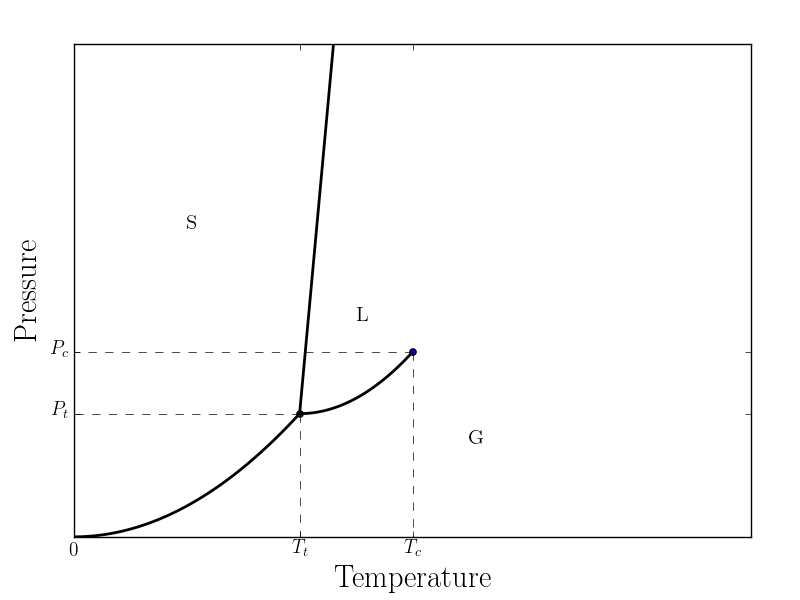
\includegraphics[width=\textwidth]{phase.png}
% 				\caption{\tiny Phase diagram of an arbitrary fluid. Labeled are the temperatures and pressures at which all three phases are present (triple point) and the critical point}
% 				\label{phase}
% 			\end{figure}
% 	\end{columns}
% \end{frame}

% \subsection*{Energy}
% 	\begin{frame}{Free energy and the burden of calculation}
% 		\begin{itemize}
% 			\item Stuff
% 		\end{itemize}
% 	\end{frame}



% \section*{Models and Methods}
% \subsection*{Models}
% \begin{frame}{Dense Fluid Models}
% \begin{columns}[t]
% 	\column{.5\textwidth}
% 		\begin{block}{Hard Sphere}	
% 			\begin{itemize}
% 				\item The hard sphere system approximates particles to have no attraction. Spheres - particles - are only allowed to undergo perfectly elastic collisions. 
% 				\item The excess internal energy is easy: either the no spheres overlap with $U_exc = 0$, or the configuration is invalid $U_{exc} = \infty$
% 			\end{itemize}
% 		\end{block}

% 	\column{.5\textwidth}
% 		\begin{block}{Square Well}	
% 			\begin{itemize}
% 		 		\item As a hard-sphere model, the spheres are not allowed to overlap.
% 		 		\item The ``square'' in square well refers to the piecewise attraction potential: $\Phi_{12} = \begin{cases} -\epsilon & \sigma \leq r \leq \lambda\\ 0 & r > \lambda\end{cases}$, where $\sigma$ is the sphere radius and $\lambda$ is the attraction range.
% 			\end{itemize}
% 		\end{block} 
% \end{columns}
% \end{frame}
% \subsection*{Methods}
% \begin{frame}{MC and TI}
% \begin{columns}[t]
% 	\column{.5\textwidth}
% 		\begin{block}{Monte-Carlo}
% 			\scriptsize \vspace{.1cm} 
% 				Monte-Carlo methods utilize random or pseudorandom sampling and check for certain conditions or measure certain quantities after a specified number of iterations. We use Transition Matrix Monte-Carlo, a broad-histogram method that efficiently determines the density of states for a given system.
% 		\end{block}
% 	\column{.5\textwidth}
% 		\begin{block}{Thermodymic Integration}
% 			\scriptsize \vspace{.1cm}
% 				Thermodynamic integration is our method to determine the . Using Monte-Carlo, we transition from a filling fraction of zero to a near-close-packed system, calculating the change in free energy at each step and eventually reaching the ``absolute'' free energy
% 		\end{block}
% \end{columns}
% \end{frame}

\end{document}
